\section{Morfometria del bacino}
\subsection{Rapporto di biforcazione e prima legge di Horton}
Dal reticolo idrografico di un bacino è possibile svolgere alcune considerazioni, come per esempio quella riguardante i suoi segmenti.\\
A seconda del numero di segmenti di cui è formato il reticolo, il bacino assume lo stesso valore di ordine, detto "ordine del bacino" ed indicato con la lettera $k$.\\
Secondo il metodo di Horton-Strahler, l'attribuzione dell'ordine al segmento del reticolo idrografico avviene mediante tre regole: 
\begin{enumerate}
    \item ai tratti iniziali (di sorgente) viene attribuito valore 1;
    \item nel caso di confluenza di due tratti di diverso ordine, al segmento a valle viene attribuito il valore maggiore tra i due;
    \item nel caso di confluenza di due tratti con ordine $x$, al segmento a valle viene attribuito un valore $x+1$.
\end{enumerate} 
\begin{figure}[H]\centering
    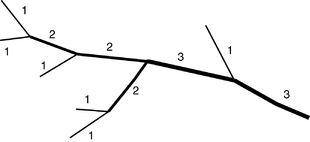
\includegraphics[scale=.75]{immagini/ordine_horton.png}
    \caption{Criterio di assegnazione dell'ordine ai segmenti del reticolo idrografico, secondo Horton-Strahler.}
    \label{ordine_horton}
\end{figure}
Avendo assegnato ad ogni tratto un certo valore numerico, è possibile conoscere la numerosità di ogni ordine.\\
Secondo la prima legge di Horton, il rapporto tra la numerosità dell'ordine precedente e la numerosità dell'ordine considerato (detto "rapporto di biforcazione parziale")
\begin{equation}
    R_u = \frac{N_{u-1}}{N_u}
\end{equation}
è statisticamente costante, e regolata dalla funzione:
\begin{equation}
    N_u= \bar{R}_b ^{(k-u)}
\end{equation}
Dove: 
\begin{itemize}
    \item $R_b$ è la media tra i rapporti di biforcazione parziali;
    \item $k$ è l'ordine del bacino;
    \item $u$ è l'ordine del tratto di reticolo considerato.
\end{itemize}
La prima legge di Horton inoltre, evidenzia come all'aumentare dell'ordine dei tratti, la lunghezza dei segmenti e le aree dei sottobacini aumentino, mentre cala la loro numerosità.\\
Nel caso del reticolo idrografico preso da noi in esame, i parametri sono: 
\begin{table}[H] \centering
    \begin{tabular}{c|c|c|c}
\toprule
    Ordine u & Segmenti Nu & Rapp. di biforcazione Rb & Nu (prima legge di Horton) \\
\midrule    
    1        & 5           &   /                     & 5.1                        \\
    2        & 2           & 2.5                      & 2.3                        \\
    3        & 1           & 2.0                      & 1.0                       \\
\bottomrule    
\end{tabular}
    \end{table}
Il rapporto di biforcazione medio $\bar{R}_b$ è pari a 2.3.\\
Interpolando i valori degli ordini dei segmenti, con la loro numerosità e con il parametro ricavato dalla prima legge di Horton, si ottiene un grafico caratteristico:
\begin{figure}[H]\centering
    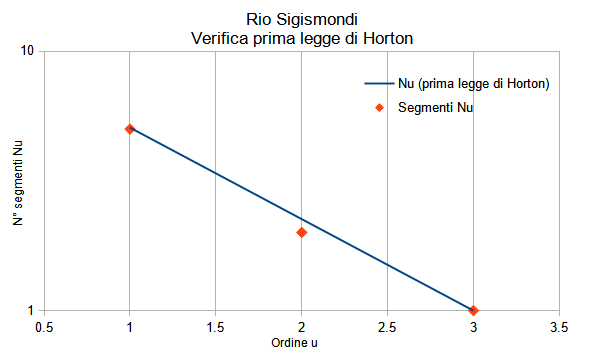
\includegraphics[scale=.75]{immagini/legge_horton.png}
    \caption{Relazione tra l'ordine del tratto, la sua numerosità e la funzione di Horton.}
    \label{legge_horton}
\end{figure}